%
% This is a borrowed LaTeX template file for lecture notes for CS267,
% Applications of Parallel Computing, UCBerkeley EECS Department.
% Now being used for CMU's 10725 Fall 2012 Optimization course
% taught by Geoff Gordon and Ryan Tibshirani.  When preparing 
% LaTeX notes for this class, please use this template.
%
% To familiarize yourself with this template, the body contains
% some examples of its use.  Look them over.  Then you can
% run LaTeX on this file.  After you have LaTeXed this file then
% you can look over the result either by printing it out with
% dvips or using xdvi. "pdflatex template.tex" should also work.
%
\documentclass[twoside]{article}
\usepackage{graphicx}
\usepackage{tikz}
\usepackage{mathpazo}
\usetikzlibrary{decorations.pathmorphing}


\setlength{\oddsidemargin}{0.25 in}
\setlength{\evensidemargin}{-0.25 in}
\setlength{\topmargin}{-0.6 in}
\setlength{\textwidth}{6.5 in}
\setlength{\textheight}{8.5 in}
\setlength{\headsep}{0.75 in}
\setlength{\parindent}{0 in}
\setlength{\parskip}{0.1 in}
%
% ADD PACKAGES here:
%
\usepackage{amsmath,amsfonts,graphicx}
%
% The following commands set up the lecnum (lecture number)
% counter and make various numbering schemes work relative
% to the lecture number.
%
\newcounter{lecnum}
\renewcommand{\thepage}{\thelecnum-\arabic{page}}
\renewcommand{\thesection}{\thelecnum.\arabic{section}}
\renewcommand{\theequation}{\thelecnum.\arabic{equation}}
\renewcommand{\thefigure}{\thelecnum.\arabic{figure}}
\renewcommand{\thetable}{\thelecnum.\arabic{table}}
%
% The following macro is used to generate the header.
%
\newcommand{\lecture}[5]{
   \pagestyle{myheadings}
   \thispagestyle{plain}
   \newpage
   \setcounter{lecnum}{#1}
   \setcounter{page}{1}
   \noindent
   \begin{center}
   \framebox{
      \vbox{\vspace{2mm}
    \hbox to 6.28in { {\bf Physics 467/667: Thermodynamics/Statistical Physics
	\hfill Spring 2017} }
       \vspace{4mm}
       \hbox to 6.28in { {\Large \hfill Lecture #1: #2  \hfill} }
       \vspace{2mm}
       \hbox to 6.28in { {\it Lecturer: #3 \hfill Scribes: #4} }
      \vspace{2mm}}
   }
   \end{center}
   \markboth{Lecture #1: #2}{Lecture #1: #2}
   \vspace*{4mm}
}
%
% Convention for citations is authors' initials followed by the year.
% For example, to cite a paper by Leighton and Maggs you would type
% \cite{LM89}, and to cite a paper by Strassen you would type \cite{S69}.
% (To avoid bibliography problems, for now we redefine the \cite command.)
% Also commands that create a suitable format for the reference list.
\renewcommand{\cite}[1]{[#1]}
\def\beginrefs{\begin{list}%
        {[\arabic{equation}]}{\usecounter{equation}
         \setlength{\leftmargin}{2.0truecm}\setlength{\labelsep}{0.4truecm}%
         \setlength{\labelwidth}{1.6truecm}}}
\def\endrefs{\end{list}}
\def\bibentry#1{\item[\hbox{[#1]}]}
%Use this command for a figure; it puts a figure in wherever you want it.
%usage: \fig{NUMBER}{SPACE-IN-INCHES}{CAPTION}
\newcommand{\fig}[3]{
			\vspace{#2}
			\begin{center}
			Figure \thelecnum.#1:~#3
			\end{center}
	}
% Use these for theorems, lemmas, proofs, etc.
\newtheorem{theorem}{Theorem}[lecnum]
\newtheorem{lemma}[theorem]{Lemma}
\newtheorem{proposition}[theorem]{Proposition}
\newtheorem{claim}[theorem]{Claim}
\newtheorem{corollary}[theorem]{Corollary}
\newtheorem{definition}[theorem]{Definition}
\newenvironment{proof}{{\bf Proof:}}{\hfill\rule{2mm}{2mm}}
% **** IF YOU WANT TO DEFINE ADDITIONAL MACROS FOR YOURSELF, PUT THEM HERE:
\newcommand\E{\mathbb{E}}
\begin{document}
%FILL IN THE RIGHT INFO.
%\lecture{**LECTURE-NUMBER**}{**DATE**}{**LECTURER**}{**SCRIBE**}
\lecture{13}{Engines and Refrigerators}{Qiang Zhu}{scribe-name1,2,3}
%\footnotetext{These notes are partially based on those of Nigel Mansell.}
% **** YOUR NOTES GO HERE:
% Some general latex examples and examples making use of the
% macros follow.  
%**** IN GENERAL, BE BRIEF. LONG SCRIBE NOTES, NO MATTER HOW WELL WRITTEN,
%**** ARE NEVER READ BY ANYBODY.

\section{Some useful equations} % Don't be this informal in your notes!
\begin{equation} \label{idealgas} PV = nRT = NkT \end{equation}
\begin{equation} \label{Avogadro} N = n \times N_A \end{equation}
\begin{equation} \label{PV-micro} PV = Nm{\overline v_x^2} = NkT\end{equation}
\begin{equation} \label{eqpartition} U_{thermal} = N \cdot f \cdot \frac{1}{2}kT \end{equation}
\begin{equation} \label{1stlaw} \Delta{U} = Q + W \end{equation}
\begin{equation} \label{work3} \Delta W = - P \Delta{V} \end{equation}
\begin{equation} \label{entropy} S = k \text{ln}\Omega \end{equation}
\begin{equation} dU = TdS - PdV  + \mu dN\end{equation}

\section{Real Heat Engines}
In the previous lecture, we have learned the theoretical limit of heat engines.
It is useful to know the upper limit when we design the engine.
However, one might also ask how it work in reality.
Can we follow the Carnot cycle in practice?

Now, let's discuss a few of engines used in real world.

\begin{figure}[ht]
\centering
\begin{tikzpicture} %[x=8cm, y=4cm]
\draw [->] (-0.5, -0.5) -- (5.0,-0.5) node[below]{$V$};
\draw [->] (-0.5, -0.5) -- (-0.5, 2.5)  node[above]{$P$};
\draw [->, line width=0.05cm, black,domain=3.0:1.5]  plot(\x, {1/((\x)^(1.4))}) node[below, xshift=0.1cm, yshift=-0.2cm] {1, Compression};
\draw [->, line width=0.05cm, blue] (1.5,0.567) -- (1.5,2.267)  node[left, yshift=-1cm]                                  {2, Ignition};
\draw [->, line width=0.05cm, black,domain=1.5:3.0]  plot(\x, {4/((\x)^(1.4))}) node[above, xshift=-0.4cm, yshift=0.5cm] {3, Power};
\draw [->, line width=0.05cm, blue] (3.0,0.859) -- (3.0,0.215)  node[right, yshift=0.4cm]                                {4, Exhaust};
\node at (1.5, -1) {$V_2$};
\node at (3.0, -1) {$V_1$};
\node  at (1.5, 3) {\large Otto cycle};

\draw [->] (9.0,-0.5) -- (14.0, -0.5) node[below]{$V$};
\draw [->] (9.0,-0.5) -- ( 9.0, 2.5) node[above]{$P$};
\draw [->, line width=0.05cm, black,domain=13.0:10.5]  plot(\x, {1/(\x-10)}) node[below, xshift=0.2cm, yshift=-1.5cm] {1, Compression};
\draw [->, line width=0.05cm, blue] (10.5,2.0) -- (11.5,2.0)  node[above, xshift=-0.8cm]                              {2, Ignition};
\draw [->, line width=0.05cm, black,domain=11.5:13.0]  plot(\x, {3/(\x-10)}) node[above, xshift=-0.5cm, yshift=0.5cm] {3, Power};
\draw [->, line width=0.05cm, blue] (13.0,1.0) -- (13.0,0.333)  node[right, yshift=0.4cm]                             {4, Exhaust};
\node at (10.5, -1) {$V_2$};
\node at (11.5, -1) {$V_3$};
\node at (13.0, -1) {$V_1$};
\node at (11.0, 3) {\large Diesel cycle};
\end{tikzpicture}
\caption{The Otto cycle and Diesel cycle.}
\end{figure}

Recall what we learned about P-V diagram in compression work, we can trivially derived the efficiency as a function of $V$
\begin{equation}
PV^{\gamma} = \text{const} ~~~~\rightarrow~~~~~~ e = 1-(\frac{V_2}{V_1})^{\gamma-1} 
                                                   = 1-\frac{T_1}{T_2} 
                                                   = 1-\frac{T_3}{T_4}~~~~~~~~~~~~~ \text{(Otto cycle)}
\end{equation}
\begin{equation}
PV = \text{const} ~~~~\rightarrow~~~~~~ e = 1-\frac{V_2}{V_1}  ~~~~~~~~~~~~~ \text{(Diesel cycle)}
\end{equation}
\\\\\\\\\\\\\\\\\\\\\\\\

Discussion on Stirling Engines
\\\\\\\\\\\\\\\\\\\\\\\\
\section{Steam Engines and Real Refrigerators}
A very different type of engine is the steam Engine, in which the liquid water/steam were used as the work substance.
It works as follows,
\begin{enumerate}
\item water is pumper to high pressure at nearly constant volume;
\item water flows into a boiler at constant pressure condition, then becomes steam;
\item steam hit the turbine, where it expands adiabatically, cools, ends up at the original pressure;
\item the fluid is cooled further to become water.
\end{enumerate}

On the other hand, refrigenator works as follows,
\begin{enumerate}
\item gas is compressed to adiabatically;
\item gives up heat and become liquids at constant pressure;
\item passes through a Throttle valve to 
\item absorbs heat and turns back to a gas in the evaproator
\end{enumerate}
\begin{figure}[ht]
\centering
\begin{tikzpicture} %[x=8cm, y=4cm]
\draw [->] (-0.5, -0.0) -- (5.0,-0.0) node[below]{$V$};
\draw [->] (-0.5, -0.0) -- (-0.5, 2.5)  node[above]{$P$};
\draw [->, line width=0.05cm]  (1.5,1.000) -- (1.5,2.267)  node[left,  yshift=-0.5cm]                                 {1, pump};
\draw [->, line width=0.05cm]  (1.5,2.267) -- (2.5,2.267)  node[above, xshift=-0.5cm]                               {2, boiler};
\draw [->, line width=0.05cm,domain=2.5:4.486]  plot(\x, {8.176/((\x)^(1.4))}) node[above, xshift=-0.4cm, yshift=0.5cm] {3, turbine};
\draw [->, line width=0.05cm] (4.486,1.000) -- (1.5,1.000)  node[below, xshift=0.8cm]                               {4, condenser};
\node  at (1.5, 3.5) {\large Rankine cycle};

\draw [->] (9.5, -0.0) -- (15.0,-0.0) node[below]{$V$};
\draw [->] (9.5, -0.0) -- (9.5, 2.5)  node[above]{$P$};
\draw [<-, line width=0.05cm]  (12.0,1.000) -- (11.5,2.267)  node[left,  yshift=-0.5cm]                                 {4, pump};
\draw [<-, line width=0.05cm]  (11.5,2.267) -- (12.5,2.267)  node[above, xshift=-0.5cm]                                 {3, condenser};
\draw [<-, line width=0.05cm,domain=12.5:14.486]  plot(\x, {8.176/((\x-10)^(1.4))}) node[above, xshift=-0.4cm, yshift=0.5cm] {2, compressor};
\draw [<-, line width=0.05cm] (14.486,1.000) -- (12.0,1.000)  node[below, xshift=0.8cm]                               {1, evaporator};
\node at (12.0, 3.5) {\large Refrigeration cycle};
\end{tikzpicture}
\caption{The Rankine cycle and Refrigeration cycle.}
\end{figure}

\begin{equation}
e = 1-\frac{Q_c}{Q_h} = 1-\frac{H_4-H_1}{H_3-H_2} = 1-\frac{H_4-H_1}{H_3-H_1}
\end{equation}

\begin{equation}
\text{COP} = \frac{Q_c}{Q_h-Q_c} = \frac{H_1-H_4}{H_2-H_3-H_1+H_4} 
\end{equation}

\section{Homework}
Problem 4.18, 4.21, 4.26, 4.27, 4.36

\end{document}

